\thispagestyle{empty}

\begin{center}

\vspace*{2cm}

\textlarger[3]{HISPARC}
\\[1em]
\textlarger[1]{RECONSTRUCTIONS}
\end{center}

\clearpage

\vspace*{\fill}

\noindent
Dutch title: \emph{HiSPARC: reconstructies.}

\vspace{1cm}

\noindent
ISBN: 153957 \\
DOI: 153957

\vspace{3cm}

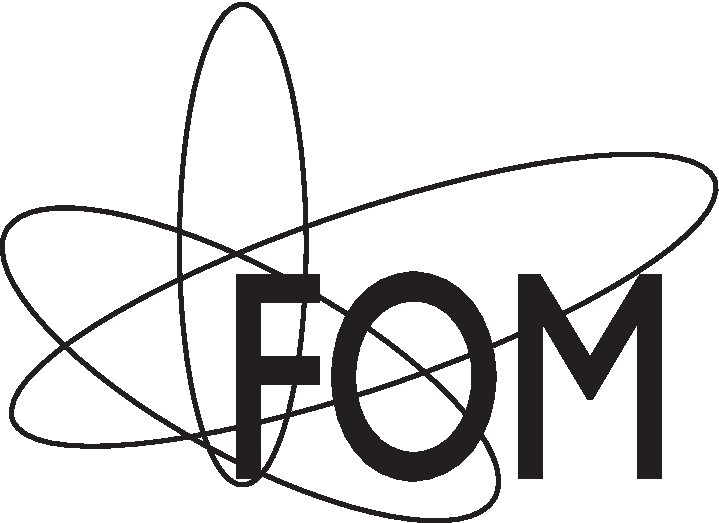
\includegraphics[height=2.5cm]{figures/logo_FOM_zw}
\hfill

\includegraphics[height=2cm]{figures/logo_NWO_zw}

\vspace{.5cm}

\noindent
This work is part of the research programme of the Foundation for
Fundamental Research on Matter (FOM), which is part of the Netherlands
Organisation for Scientific Research (NWO).  It was carried out at the
National Institute for Subatomic Physics (Nikhef).


% Actual 'titlepage'

\cleardoublepage
\thispagestyle{empty}

\begin{center}

\vspace*{2cm}

\textlarger[3]{HISPARC}
\\[1em]
\textlarger[1]{RECONSTRUCTIONS}


\begin{onehalfspace}

\vspace{2cm}

PROEFSCHRIFT

\vspace{2cm}

.....\\

\vspace{1cm}

door

\vspace{1cm}

Adriaan Paul Ludovic Siem de Laat\\
geboren op 16 september 1987\\
te Amsterdam

\end{onehalfspace}
\end{center}


\newpage


\noindent
Dit proefschrift is nog niet goedgekeurd.
\begin{tabbing}
Promotor: \\
Assistent-promotor: 
\end{tabbing}
